\documentclass[10pt, aspectratio=169]{beamer}
\usepackage{natbib}
\usepackage{bibentry}
\nobibliography*

\usepackage{color, xcolor}
\definecolor{mydarkblue}{rgb}{0,0.08,0.45}
\definecolor{mydarkred}{HTML}{990000}
\definecolor{metropolisdark}{RGB}{35,35,59}

\usepackage{hyperref}
\hypersetup{
    colorlinks=true,
    citecolor=mydarkred,
    linkcolor=metropolisdark,
    urlcolor=mydarkblue
}

\usetheme[progressbar=frametitle]{metropolis}
\metroset{block=fill}
\usepackage{appendixnumberbeamer}
\usepackage{multicol}

\usepackage[absolute,overlay]{textpos}

\usepackage{nccmath}
\usepackage{caption}
\usepackage{booktabs}
\usepackage[scale=2]{ccicons}

% \usepackage{pgfplots}
% \usepgfplotslibrary{dateplot}

% Math macros to be imported into main.tex

\def\xx{{\boldsymbol x}}
\def\qq{{\boldsymbol q}}
\def\dd{{\boldsymbol d}}
\def\XX{{\boldsymbol X}}
\def\YY{{\boldsymbol Y}}
\def\ZZ{{\boldsymbol Z}}
\def\aa{{\boldsymbol a}}
\def\bb{{\boldsymbol b}}
\def\rr{{\boldsymbol r}}
\def\cc{{\boldsymbol c}}
\def\qq{{\boldsymbol q}}
\def\WW{{\boldsymbol W}}
\def\KK{{\boldsymbol K}}
\def\II{{\boldsymbol I}}
\def\yy{{\boldsymbol y}}
\def\vv{{\boldsymbol v}}
\def\uu{{\boldsymbol u}}
\def\ww{{\boldsymbol w}}
\def\zz{{\boldsymbol z}}
\def\SS{{\boldsymbol S}}
\def\BB{{\boldsymbol B}}
\def\AA{{\boldsymbol A}}
\def\CC{{\boldsymbol C}}
\def\GG{{\boldsymbol G}}
\def\FF{{\boldsymbol F}}
\def\MM{{\boldsymbol M}}
\def\DD{{\boldsymbol D}}
\def\PP{{\boldsymbol P}}
\def\TT{{\boldsymbol T}}
\def\VV{{\boldsymbol V}}
\def\OO{{\boldsymbol O}}
\def\LL{{\boldsymbol L}}
\def\HH{{\boldsymbol H}}
\def\bphi{{\boldsymbol \phi}}
\def\QQ{{\boldsymbol Q}}
\def\UU{{\boldsymbol U}}
\def\HH{{\boldsymbol H}}
\def\XX{{\boldsymbol X}}
\def\Id{{\boldsymbol{I}}}
\def\bQQ{{\textcolor{blue}{\boldsymbol Q_n}}}
\def\bbQQ{{\textcolor{blue}{\boldsymbol Q_n^{(1)}}}}
\def\rQQ{{\textcolor{red}{\boldsymbol Q}}}

\def\balpha{{\boldsymbol \alpha}}
\def\bpsi{{\boldsymbol \psi}}
\def\ttheta{{\boldsymbol \theta}}
\def\LLambda{{\boldsymbol \Lambda}}
\def\SSigma{{\boldsymbol \Sigma}}

\def\eeps{{\boldsymbol \varepsilon}}
\def\eeta{{\boldsymbol \eta}}
\def\g{{g}}
\def\ee{{\boldsymbol e}}

\def\dif{\mathop{}\!\mathrm{d}}
\def\Proba{\mathbb{P}}
\def\MP{\mu_{\mathrm{MP}}}
\def\RR{{\mathbb R}}
\def\EE{{\mathbb E}\,}
\newcommand{\Econd}{\mathbf{E}}
\renewcommand{\vec}{\mathbf{vec}}
\DeclareMathOperator{\prox}{\mathbf{prox}}
\DeclareMathOperator{\tr}{tr}
\def\defas{\stackrel{\text{def}}{=}}
\DeclareMathOperator*{\dom}{dom}
\DeclareMathOperator*{\supp}{supp}
\DeclareMathOperator*{\Fix}{Fix}
\DeclareMathOperator*{\Var}{Var}
\DeclareMathOperator*{\argmin}{{arg\,min}}
\DeclareMathOperator*{\minimize}{minimize}
\DeclareMathOperator*{\diag}{\mathbf{diag}}

\newcommand{\Prto}[1]{
  { \xrightarrow[ #1 \to \infty]{\Pr }}
}

% \DeclareDocumentCommand{\Asto} {o} {
%   \IfNoValueTF {#1}
%   {\overset{\text{\rm a.s.}}{\longrightarrow}}
%   { \xrightarrow[ #1 \to \infty]{\text{\rm a.s.} }}
% }

\newcommand{\blue}{\color{blue}}

\definecolor{myblue}{HTML}{D2E4FC}
\newcommand*\mybluebox[1]{\colorbox{myblue}{\hspace{1em}#1\hspace{1em}}}

% !TEX root = non_convex_Courtney.tex

% Macros for the Non-Convex Catalyst Paper

%% !TEX root = non_convex_Courtney.tex

% Macros for the Non-Convex Catalyst Paper

%% !TEX root = non_convex_Courtney.tex

% Macros for the Non-Convex Catalyst Paper

%\input{macros}

\newcommand{\vs}{}
%\newcommand{\vs}{\vspace*{0.0cm}}
\newcommand{\cnt}{k}
\newcommand{\pr}{{\rm prox}}
\newcommand{\eg}{\emph{e.g.}}

\renewcommand\epsilon\varepsilon
%\newcommand{\dom}{\textrm{dom }} %counter
\newcommand{\smthpara}{\kappa} % the smoothing parameter 
\newcommand{\smthparacvx}{\kappa_{\text{\rm cvx}}} % the smoothing
                                % parameter  convex
\newcommand{\smthparainit}{\kappa_0} 
\newcommand{\env}{f_{\smthpara}}
 % envelope of the prox; f_\kappa(x; y) = f(x) + kappa/2 ||x-y||^2
\newcommand{\accx}{\tilde{x}} %the \acc_x \approx argmin f_{\kappa}(x;y_k)
\newcommand{\proxx}{\bar{x}} %the \proxx \approx argmin f_{\kappa}(x;
                             %x_{k-1})
\newcommand{\bproxx}{\bar{x}^{b}} %the \proxx \approx argmin f_{\kappa}(x;
                         
                            %x_{k-1})
%\newcommand{\prox}{p_{\frac{1}{\smthpara} f}} %writes prox: kappa f ->
                                %1/kappa f
% \newcommand{\prox}{\text{prox}} 
\newcommand{\weakcnx}{\rho} %weak convexity parameter
% \newcommand{\argmin}{\operatornamewithlimits{argmin}} %argmin
\newcommand{\sccnt}{i} %Outer counter for strong convexity
\newcommand{\scnx}{\mu} %Strong convexity constant
\newcommand{\smth}{L} %smooth parameter \beta->L
\newcommand{\globalcnt}{b} %global counter for complexity
\newcommand{\li}{\operatornamewithlimits{liminf}} %argmin
%\newcommand{\mtd}{\mathcal{M}} %optimization method M used as sub-routine

%% Strong Convexity w/ Estimate Sequences %%%%%%%%%%
\newcommand{\estseqpara}{\lambda} %Estimating sequence constants
\newcommand{\estseq}{\Phi} %Estimating sequence functions
\newcommand{\estseqquad}{\gamma} %Constant multiplied by the
                                %quad. term in estimating sequence
\newcommand{\estseqcenter}{\estseq^*} % center of the estimating sequence
%% General Math %%%%%%%%%%%%%%
\newcommand{\ip}[1] {\langle #1 \rangle } %inner product
\newcommand{\norm}[1] {\left \| #1 \right \|} %norm
\newcommand{\dist}{{\rm dist}} %distance
\newcommand{\R}{{\mathbb R}} %Real numbers
\newcommand{\N}{{\mathbb N}} %Natural numbers
\newcommand{\mtd}{{\mathcal M}} %Optimization method M
\newcommand{\proxi}{\text{prox}} %proximal operator
\newcommand{\Real}{{\mathbb R}} %Real numbers
\newcommand{\oR}{\overline \R} %Reals + infinity


%%%%%%%%% Theorems %%%%%%%%%%%%%
%\newtheorem{claim}{Claim}
%\newtheorem{theorem}{Theorem}[section]
%\newtheorem{proposition}[theorem]{Proposition}
%\newtheorem{lemma}[theorem]{Lemma}
%\newtheorem{defn}[theorem]{Definition}
%\newtheorem{corollary}{Corollary}[section]
%\newtheorem{pa}{Part}
%\newtheorem{subclaim}{Subclaim}
%\newtheorem{example}{Example}[section]

%%%Random stuff%%%
\newcommand{{\newalgosp}}{Basic 4WD-Catalyst~}%basic algo, with small space after the name
\newcommand{{\newalgo}}{Basic 4WD-Catalyst}%basic algo, no space
\newcommand{{\autonewalgosp}}{4WD-Catalyst~}%adaptive algo, with small space after the name , it was before 4WD-Catalyst-Automatic
\newcommand{{\autonewalgo}}{4WD-Catalyst}%adaptive algo, no space it was before 4WD-Catalyst-Automatic
\newcommand{\linesearch}{{Auto-adapt}}

\newcommand{\mylabel}[2]{#2\def\@currentlabel{#2}\label{#1}}
\newcommand{\mynote}[1]{{\bf \color{blue}{#1} }\\}


\newcommand{\vs}{}
%\newcommand{\vs}{\vspace*{0.0cm}}
\newcommand{\cnt}{k}
\newcommand{\pr}{{\rm prox}}
\newcommand{\eg}{\emph{e.g.}}

\renewcommand\epsilon\varepsilon
%\newcommand{\dom}{\textrm{dom }} %counter
\newcommand{\smthpara}{\kappa} % the smoothing parameter 
\newcommand{\smthparacvx}{\kappa_{\text{\rm cvx}}} % the smoothing
                                % parameter  convex
\newcommand{\smthparainit}{\kappa_0} 
\newcommand{\env}{f_{\smthpara}}
 % envelope of the prox; f_\kappa(x; y) = f(x) + kappa/2 ||x-y||^2
\newcommand{\accx}{\tilde{x}} %the \acc_x \approx argmin f_{\kappa}(x;y_k)
\newcommand{\proxx}{\bar{x}} %the \proxx \approx argmin f_{\kappa}(x;
                             %x_{k-1})
\newcommand{\bproxx}{\bar{x}^{b}} %the \proxx \approx argmin f_{\kappa}(x;
                         
                            %x_{k-1})
%\newcommand{\prox}{p_{\frac{1}{\smthpara} f}} %writes prox: kappa f ->
                                %1/kappa f
% \newcommand{\prox}{\text{prox}} 
\newcommand{\weakcnx}{\rho} %weak convexity parameter
% \newcommand{\argmin}{\operatornamewithlimits{argmin}} %argmin
\newcommand{\sccnt}{i} %Outer counter for strong convexity
\newcommand{\scnx}{\mu} %Strong convexity constant
\newcommand{\smth}{L} %smooth parameter \beta->L
\newcommand{\globalcnt}{b} %global counter for complexity
\newcommand{\li}{\operatornamewithlimits{liminf}} %argmin
%\newcommand{\mtd}{\mathcal{M}} %optimization method M used as sub-routine

%% Strong Convexity w/ Estimate Sequences %%%%%%%%%%
\newcommand{\estseqpara}{\lambda} %Estimating sequence constants
\newcommand{\estseq}{\Phi} %Estimating sequence functions
\newcommand{\estseqquad}{\gamma} %Constant multiplied by the
                                %quad. term in estimating sequence
\newcommand{\estseqcenter}{\estseq^*} % center of the estimating sequence
%% General Math %%%%%%%%%%%%%%
\newcommand{\ip}[1] {\langle #1 \rangle } %inner product
\newcommand{\norm}[1] {\left \| #1 \right \|} %norm
\newcommand{\dist}{{\rm dist}} %distance
\newcommand{\R}{{\mathbb R}} %Real numbers
\newcommand{\N}{{\mathbb N}} %Natural numbers
\newcommand{\mtd}{{\mathcal M}} %Optimization method M
\newcommand{\proxi}{\text{prox}} %proximal operator
\newcommand{\Real}{{\mathbb R}} %Real numbers
\newcommand{\oR}{\overline \R} %Reals + infinity


%%%%%%%%% Theorems %%%%%%%%%%%%%
%\newtheorem{claim}{Claim}
%\newtheorem{theorem}{Theorem}[section]
%\newtheorem{proposition}[theorem]{Proposition}
%\newtheorem{lemma}[theorem]{Lemma}
%\newtheorem{defn}[theorem]{Definition}
%\newtheorem{corollary}{Corollary}[section]
%\newtheorem{pa}{Part}
%\newtheorem{subclaim}{Subclaim}
%\newtheorem{example}{Example}[section]

%%%Random stuff%%%
\newcommand{{\newalgosp}}{Basic 4WD-Catalyst~}%basic algo, with small space after the name
\newcommand{{\newalgo}}{Basic 4WD-Catalyst}%basic algo, no space
\newcommand{{\autonewalgosp}}{4WD-Catalyst~}%adaptive algo, with small space after the name , it was before 4WD-Catalyst-Automatic
\newcommand{{\autonewalgo}}{4WD-Catalyst}%adaptive algo, no space it was before 4WD-Catalyst-Automatic
\newcommand{\linesearch}{{Auto-adapt}}

\newcommand{\mylabel}[2]{#2\def\@currentlabel{#2}\label{#1}}
\newcommand{\mynote}[1]{{\bf \color{blue}{#1} }\\}


\newcommand{\vs}{}
%\newcommand{\vs}{\vspace*{0.0cm}}
\newcommand{\cnt}{k}
\newcommand{\pr}{{\rm prox}}
\newcommand{\eg}{\emph{e.g.}}

\renewcommand\epsilon\varepsilon
%\newcommand{\dom}{\textrm{dom }} %counter
\newcommand{\smthpara}{\kappa} % the smoothing parameter 
\newcommand{\smthparacvx}{\kappa_{\text{\rm cvx}}} % the smoothing
                                % parameter  convex
\newcommand{\smthparainit}{\kappa_0} 
\newcommand{\env}{f_{\smthpara}}
 % envelope of the prox; f_\kappa(x; y) = f(x) + kappa/2 ||x-y||^2
\newcommand{\accx}{\tilde{x}} %the \acc_x \approx argmin f_{\kappa}(x;y_k)
\newcommand{\proxx}{\bar{x}} %the \proxx \approx argmin f_{\kappa}(x;
                             %x_{k-1})
\newcommand{\bproxx}{\bar{x}^{b}} %the \proxx \approx argmin f_{\kappa}(x;
                         
                            %x_{k-1})
%\newcommand{\prox}{p_{\frac{1}{\smthpara} f}} %writes prox: kappa f ->
                                %1/kappa f
% \newcommand{\prox}{\text{prox}} 
\newcommand{\weakcnx}{\rho} %weak convexity parameter
% \newcommand{\argmin}{\operatornamewithlimits{argmin}} %argmin
\newcommand{\sccnt}{i} %Outer counter for strong convexity
\newcommand{\scnx}{\mu} %Strong convexity constant
\newcommand{\smth}{L} %smooth parameter \beta->L
\newcommand{\globalcnt}{b} %global counter for complexity
\newcommand{\li}{\operatornamewithlimits{liminf}} %argmin
%\newcommand{\mtd}{\mathcal{M}} %optimization method M used as sub-routine

%% Strong Convexity w/ Estimate Sequences %%%%%%%%%%
\newcommand{\estseqpara}{\lambda} %Estimating sequence constants
\newcommand{\estseq}{\Phi} %Estimating sequence functions
\newcommand{\estseqquad}{\gamma} %Constant multiplied by the
                                %quad. term in estimating sequence
\newcommand{\estseqcenter}{\estseq^*} % center of the estimating sequence
%% General Math %%%%%%%%%%%%%%
\newcommand{\ip}[1] {\langle #1 \rangle } %inner product
\newcommand{\norm}[1] {\left \| #1 \right \|} %norm
\newcommand{\dist}{{\rm dist}} %distance
\newcommand{\R}{{\mathbb R}} %Real numbers
\newcommand{\N}{{\mathbb N}} %Natural numbers
\newcommand{\mtd}{{\mathcal M}} %Optimization method M
\newcommand{\proxi}{\text{prox}} %proximal operator
\newcommand{\Real}{{\mathbb R}} %Real numbers
\newcommand{\oR}{\overline \R} %Reals + infinity


%%%%%%%%% Theorems %%%%%%%%%%%%%
%\newtheorem{claim}{Claim}
%\newtheorem{theorem}{Theorem}[section]
%\newtheorem{proposition}[theorem]{Proposition}
%\newtheorem{lemma}[theorem]{Lemma}
%\newtheorem{defn}[theorem]{Definition}
%\newtheorem{corollary}{Corollary}[section]
%\newtheorem{pa}{Part}
%\newtheorem{subclaim}{Subclaim}
%\newtheorem{example}{Example}[section]

%%%Random stuff%%%
\newcommand{{\newalgosp}}{Basic 4WD-Catalyst~}%basic algo, with small space after the name
\newcommand{{\newalgo}}{Basic 4WD-Catalyst}%basic algo, no space
\newcommand{{\autonewalgosp}}{4WD-Catalyst~}%adaptive algo, with small space after the name , it was before 4WD-Catalyst-Automatic
\newcommand{{\autonewalgo}}{4WD-Catalyst}%adaptive algo, no space it was before 4WD-Catalyst-Automatic
\newcommand{\linesearch}{{Auto-adapt}}

\newcommand{\mylabel}[2]{#2\def\@currentlabel{#2}\label{#1}}
\newcommand{\mynote}[1]{{\bf \color{blue}{#1} }\\}

\usepackage{minted}
\usepackage[version=4]{mhchem}

\usepackage{tikz}
\usetikzlibrary{shadows,calc,backgrounds,matrix,fit}



% code adapted from https://tex.stackexchange.com/a/11483/3954

% some parameters for customization
\def\shadowshift{3pt,-3pt}
\def\shadowradius{6pt}

\colorlet{innercolor}{black!60}
\colorlet{outercolor}{gray!05}

% this draws a shadow under a rectangle node
\newcommand\drawshadow[1]{
    \begin{pgfonlayer}{shadow}
        \shade[outercolor,inner color=innercolor,outer color=outercolor] ($(#1.south west)+(\shadowshift)+(\shadowradius/2,\shadowradius/2)$) circle (\shadowradius);
        \shade[outercolor,inner color=innercolor,outer color=outercolor] ($(#1.north west)+(\shadowshift)+(\shadowradius/2,-\shadowradius/2)$) circle (\shadowradius);
        \shade[outercolor,inner color=innercolor,outer color=outercolor] ($(#1.south east)+(\shadowshift)+(-\shadowradius/2,\shadowradius/2)$) circle (\shadowradius);
        \shade[outercolor,inner color=innercolor,outer color=outercolor] ($(#1.north east)+(\shadowshift)+(-\shadowradius/2,-\shadowradius/2)$) circle (\shadowradius);
        \shade[top color=innercolor,bottom color=outercolor] ($(#1.south west)+(\shadowshift)+(\shadowradius/2,-\shadowradius/2)$) rectangle ($(#1.south east)+(\shadowshift)+(-\shadowradius/2,\shadowradius/2)$);
        \shade[left color=innercolor,right color=outercolor] ($(#1.south east)+(\shadowshift)+(-\shadowradius/2,\shadowradius/2)$) rectangle ($(#1.north east)+(\shadowshift)+(\shadowradius/2,-\shadowradius/2)$);
        \shade[bottom color=innercolor,top color=outercolor] ($(#1.north west)+(\shadowshift)+(\shadowradius/2,-\shadowradius/2)$) rectangle ($(#1.north east)+(\shadowshift)+(-\shadowradius/2,\shadowradius/2)$);
        \shade[outercolor,right color=innercolor,left color=outercolor] ($(#1.south west)+(\shadowshift)+(-\shadowradius/2,\shadowradius/2)$) rectangle ($(#1.north west)+(\shadowshift)+(\shadowradius/2,-\shadowradius/2)$);
        \filldraw ($(#1.south west)+(\shadowshift)+(\shadowradius/2,\shadowradius/2)$) rectangle ($(#1.north east)+(\shadowshift)-(\shadowradius/2,\shadowradius/2)$);
    \end{pgfonlayer}
}

% create a shadow layer, so that we don't need to worry about overdrawing other things
\pgfdeclarelayer{shadow} 
\pgfsetlayers{shadow,main}

\newsavebox\mybox
\newlength\mylen

\newcommand\shadowimage[2][]{%
\setbox0=\hbox{\includegraphics[#1]{#2}}
\setlength\mylen{\wd0}
\ifnum\mylen<\ht0
\setlength\mylen{\ht0}
\fi
\divide \mylen by 120
\def\shadowshift{\mylen,-\mylen}
\def\shadowradius{\the\dimexpr\mylen+\mylen+\mylen\relax}
\begin{tikzpicture}
\node[anchor=south west,inner sep=0] (image) at (0,0) {\includegraphics[#1]{#2}};
\drawshadow{image}
\end{tikzpicture}}

\usepackage{xspace}
\newcommand{\themename}{\textbf{\textsc{metropolis}}\xspace}

\definecolor{myorange}{RGB}{217,95,2}
\definecolor{mycolor2}{RGB}{231,138,195}
\definecolor{mycolor3}{RGB}{255,217,47}
\definecolor{mybrown}{RGB}{166,86,40}


\title{Random Matrix Theory for Machine Learning}
\subtitle{{\bfseries Part 1}: Motivating Questions and Building Blocks}
% \date{\today}
\date{}
\author{\underline{Fabian Pedregosa}$^1$, Courtney Paquette$^{1, 2}$, Tom Trogdon$^3$, Jeffrey Pennington$^1$}
\institute{
$^1$ Google Research\,, $^2$ McGill University\,, $^3$ University of Washington\\
\\
\url{https://random-matrix-learning.github.io}
}
% \titlegraphic{\hfill\includegraphics[height=1.5cm]{logo.pdf}}

\begin{document}
\maketitle

\begin{frame}{About this tutorial}

{\bfseries Objective}:
\begin{itemize}
    \item Applications of \emph{Random Matrix Theory} (RMT) in Machine Learning.
    \item Proof techniques in RMT
\end{itemize}

\pause
{\bfseries Structure}:
\begin{enumerate}
    \item Motivating Questions and Building Blocks, \emph{Fabian Pedregosa}
    \item Introduction to Random Matrix Theory, \emph{Courtney Paquette}
    \item Analysis of Numerical Algorithms, \emph{Tom Trogdon}
    \item The Mystery of Generalization: Why Does Deep Learning Work?, \emph{Jeffrey Pennington}
\end{enumerate}

\begin{center}
    \url{https://random-matrix-learning.github.io}
\end{center}

\end{frame}

% \begin{frame}{Table of contents}
%   \setbeamertemplate{section in toc}[sections numbered]
%   \tableofcontents%[hideallsubsections]
% \end{frame}


% like Tropp: https://youtu.be/bwTUe5a8JZk?t=187


\begin{frame}{What is a Random Matrix?}
    A \emph{random matrix} is a matrix whose entries are random variables, not necessarily independent.
    
    \pause\begin{exampleblock}{Example}
    Realization of a random matrix:
    $$
    \boldsymbol{Z} = \begin{bmatrix}
1.066 &  0.908 &  1.026 & -0.294 &  0.879\\
        0.908 & -1.794 &  0.596 & -1.014 & -0.103\\
       1.026 &  0.596 & -0.246 &  0.968 &  0.750 &\\
       -0.294 & -1.014 &  0.968 &  0.184&  0.812 & \\
       0.879 &  -0.103 &   0.750 &   0.812 &   0.210  & \\
\end{bmatrix}
    $$
    \end{exampleblock}
    
    \pause
    {\bfseries Goal} of Random Matrix Theory is to understand their
    \begin{multicols}{3}
    \begin{itemize}
    \item eigenvalues
    \item eigenvectors
    \item norms
    \item singular values
    \item singular vectors
    \item \ldots
    \end{itemize}
    \end{multicols}
\end{frame}



\section{Where do Random Matrices\\ Come From?}

\begin{frame}{1928: Eigenvalues of Normal Covariance Matrices}
\note{From the statistics field}

\begin{center}
\shadowimage[width=0.6\linewidth]{part-1-images/wishart_biometrika.png}
\end{center}
{\begin{columns}
    \begin{column}{0.25\textwidth}
    \begin{center}
    \shadowimage[width=0.5\linewidth]{part-1-images/JohnWishart.jpg}\\
    ~~John Wishart
    \end{center}
    \end{column}
    \begin{column}{0.6\textwidth}
    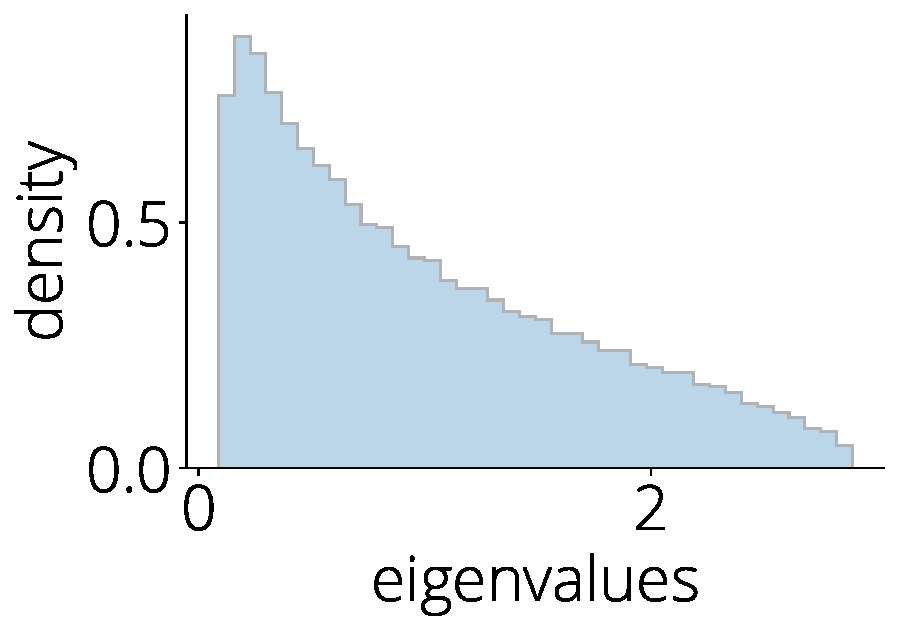
\includegraphics[width=0.55\linewidth]{part-1-images/wishart.pdf}
    \end{column}
\end{columns}}
\pause
{\begin{align*}
\boldsymbol{W} = \boldsymbol{X} \boldsymbol{X}^{\top}\,, X_{ij} &\sim \mathcal{N}(0, 1) \\
p(\lambda_1, \ldots, \lambda_N) &\propto e^{-\frac{1}{2}\sum_i\lambda_i}\prod \lambda_i^{(n-p-1)/2}\prod_{i<j}|\lambda_i-\lambda_j|
\end{align*}}
\nocite{wishart1928generalised}
\end{frame}



% \begin{frame}{1951: Random Matrix Theory and Numerical Linear Algebra}
% \begin{columns}
%     \begin{column}{0.25\textwidth}
%     \center\shadowimage[width=0.6\linewidth]{part-1-images/JohnvonNeumann.png}\\
%     {\small John von Neumann}\\
%     \vspace*{1em}\shadowimage[width=0.6\linewidth]{part-1-images/Herman_Goldstine.jpg}\\
%     {\small Herman Goldstine}
%     \vspace*{1em}\end{column}

%     \begin{column}{0.6\textwidth}
%     \shadowimage[width=\linewidth]{part-1-images/neumann_goldstine.png} \\
%     \vspace*{3em}\shadowimage[width=\linewidth]{part-1-images/vonneumann_excerpt.png}
%     \end{column}
% \end{columns}
% \nocite{goldstine1951numerical}
% \end{frame}



\begin{frame}{1955: Random Symmetric Matrices}
\note{Although RMT was only introduced from the statistics community, it really took off by physicists. }
\begin{center}
{\centering\shadowimage[width=0.5\linewidth]{part-1-images/wigner_paper.png}}
\end{center}

\begin{columns}
\begin{column}{0.2\linewidth}
% \begin{tikzpicture}
% \path (-2,-2) rectangle (2,2);
% \pgfmathdeclarerandomlist{color}{{red}{white}}
% \pgfmathsetseed{1}
% \foreach \A/\R in {25/1,12/0.9,15/0.8,20/0.7,12/0.5,7/0.3,1/0}{
%       \pgfmathsetmacro{\S}{360/\A}
%           \foreach \B in {0,\S,...,360}{
%               \pgfmathrandomitem{\C}{color}
%               \shade[ball color=\C] (\B+\A:\R) circle (5pt);
%           }
% }
% \node at (-1,1.3) {\ce{^{238}U}};
% \end{tikzpicture}
\begin{center}
\center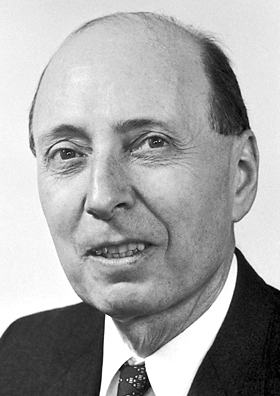
\includegraphics[width=0.7\linewidth]{part-1-images/Wigner.jpg}\\
Eugene Wigner
\end{center}
\end{column}
\begin{column}{0.5\linewidth}
\center\shadowimage[width=0.6\linewidth]{part-1-images/gadolinium-156.png}\\
\center\shadowimage[width=0.5\linewidth]{part-1-images/nuclei_spacing.png}\\
\end{column}
\begin{column}{0.3\linewidth}
{\footnotesize Energy levels of heavy nuclei, compared with the random matrix theory prediction.\\
Source: \citep{PhysRev.120.1698}}\\
\end{column}
\end{columns}
\nocite{wigner1955characteristic}
\end{frame}



\begin{frame}{Model for high-dimensional phenomena}
\begin{columns}
\begin{column}{0.5\linewidth}
\begin{itemize}
    \item Number Theory \citep{montgomery1973pair, keating1993riemann}. 
    \item Graph Theory \citep{erdos1960evolution}.
    \item Finance \citep{bouchaud2009financial}.
    % \item Transportation system \citep{krbalek2000statistical, jagannath2017random}
    
    \item Wireless communication \citep{tulino2004random}
    \item Machine Learning ...
\end{itemize}
\end{column}
\begin{column}{0.5\linewidth}
\begin{center}
\shadowimage[width=0.8\linewidth]{part-1-images/gaps_riemann.png}\\
\end{center}
{\scriptsize Distribution function of gaps between eigenvalues
compared with histogram of gaps between $\zeta$ zeros. Source: \citep{odlyzko1987distribution}}
\end{column}
\end{columns}


% \pause Faster algorithms for
%     \begin{itemize}
%     \item Randomized Linear Algebra \citep{halko2011finding, drineas2018lectures, gower2015randomized}
    
%     \item Kernel methods \citep{williams2001using, drineas2005nystrom, rudi2015less}
    
%     \item Sparsification \citep{spielman2011spectral}
    
%     \item ...
% \end{itemize}

\end{frame}


\begin{frame}{Random Matrices in Machine Learning: Loss Landscape}
\note{

In the early days of neural nets (late
1980s and early 1990s), many researchers and engineers were experimenting with relatively small networks, whose convergence tends to be unreliable, particularly when using batch optimization. Multilayer
neural nets earned a reputation of being finicky and
unreliable, which in part caused the community to focus on simpler method with convex loss functions, such
as kernel machines and boosting.

However, several researchers experimenting with larger
networks and SGD had noticed that, while multilayer
nets do have many local minima, the result of multiple experiments consistently give very similar performance. This suggests that, while local minima are
numerous, they are relatively easy to find, and they
are all more or less equivalent in terms of performance
on the test set.

To explain this phenomena

the spinglass model originates from condensed matter physics
where it is used to represent a magnet with irregularly aligned spins

They discovered and proved the existence of a layered structure
of the low critical values for the model’s Hamiltonian which in fact is a Gaussian process

 random Gaussian functions on the N-dimensional sphere, known as p-spin spherical spin glass
models in the physics literature and as isotropic models in the Gaussian process literature
}

% \begin{itemize}
%     \item Early days ('80s, '90s): small networks, unreliable.
%     \item 2010s: larger networks + SGD. Consistent good performance.
% \end{itemize}

\begin{exampleblock}{Spin Glass model of the Loss Landscape}
Early: {\scriptsize\citep{amit1985spin, gardner1988optimal, dotsenko1995introduction}} \\
Late: {\scriptsize\citep{dauphin2014identifying, sagun2014explorations, choromanska2015loss, baity2018comparing}}
\end{exampleblock}
\begin{figure}
    \centering
    \shadowimage[width=0.8\linewidth]{part-1-images/spinglass.png}
    \caption*{{\bfseries Loss study through spin-glass model}. Scaled test losses for the spin-glass (left) and the neural network (right). Source: \citet{choromanska2015loss} \emph{The Loss Surfaces of Multilayer Networks}.}
    \label{fig:my_label}
\end{figure}
% \pause\vspace*{-1em}{\small
% % \citet{}, \emph{Identifying and attacking the saddle point problem in
% % high-dimensional non-convex optimization}\\
% % \citet{choromanska2015loss} \\
% }
\end{frame}

% \begin{frame}{Random Matrices in Machine Learning: Loss Landscape}
% \begin{columns}
% \begin{column}{0.4\linewidth}
% {\small \citet{martin2018implicit} \emph{Implicit Self-Regularization in Deep Neural Networks: Evidence
% from Random Matrix Theory and Implications for Learning}}
% \end{column}
%     \begin{column}{0.6\linewidth}
%     \vspace*{1em}\shadowimage[width=0.8\linewidth]{part-1-images/martin_fig1.png}
%     \shadowimage[width=0.8\linewidth]{part-1-images/martin_fig2.png}
% \end{column}
% \end{columns}
% \begin{center}
% \end{center}
% \end{frame}

\begin{frame}{Random Matrices in Machine Learning: Loss Landscape}
\note{
Recently, with new methods that scale and allow us to compute the full spectrum of the Hessian
}

\begin{columns}
\begin{column}{0.5\linewidth}
 New methods and software$^{1, 2, 3}$ to compute Hessian eigenvalues of large models  \citep{ghorbani2019investigation, yao2020pyhessian, JMLR:v21:20-933}
 
 
\vspace*{2em}{\scriptsize 
$^1$ \url{https://github.com/amirgholami/PyHessian}\\
$^2$ \url{https://github.com/google/spectral-density/}\\
$^3$ \url{https://github.com/deep-lab/DeepnetHessian}\\
}

\only<2>{\vspace*{2em}{RMT model for the Hessian still an open problem \citep{Liao2021, baskerville2021applicability} ...}}

% \pause\vspace*{1em} Formal theory for neural networks with random weights \citep{pennington2017nonlinear, peche2019note}
\end{column}
\begin{column}{0.5\linewidth}
  \shadowimage[width=0.7\linewidth]{part-1-images/papyan_fig2.png}\\
  \vspace*{-0.5em}{\small \quad Source: \citep{JMLR:v21:20-933} }
\end{column}
\end{columns}
 
\end{frame}


\begin{frame}{Random Matrices in Machine Learning: Numerical Algorithms}

% \textcolor{red}{TODO: simplify}

Analyze algorithms with {\bfseries random}  data.
\begin{columns}
\begin{column}{0.5\linewidth}
\begin{itemize}
    \item Simplex {\footnotesize\citep{Borgwardt1987, Smale1983, Spielman2004, Vershynin2009a} etc}.
    \item Conjugate Gradient {\footnotesize\citep{Deift2017, paquette2020universality}}
    \item Acceleration {\footnotesize\citep{pedregosa2020acceleration, lacotte2020optimal}}
    % \pause\item Universality. {\footnotesize\citep{deift2014universality, sagun2015universal}}
\end{itemize}
\end{column}
\begin{column}{0.5\linewidth}
\begin{center}
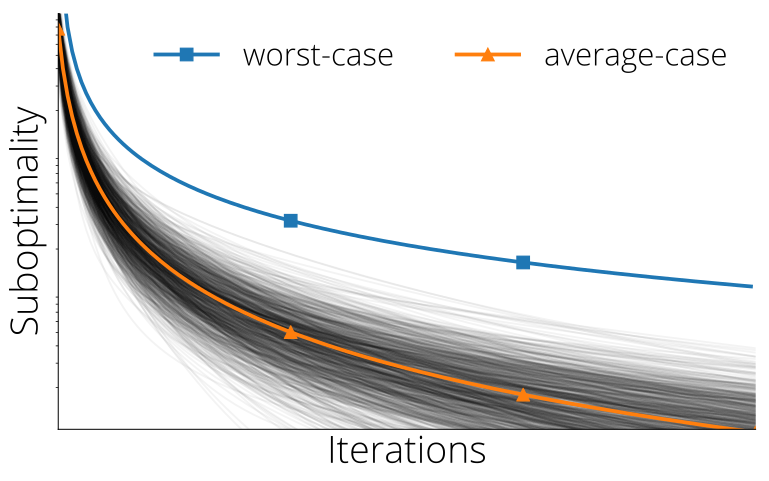
\includegraphics[width=0.9\linewidth]{part-1-images/averagecase.png}
\end{center}
% {\footnotesize{\bfseries Halting Time Universality.}} {\scriptsize Source: \citet{sagun2015universal} \emph{ Universal halting times in optimization and machine learning}}
\end{column}
\end{columns}
\pause\vspace*{1em}{Topic of Part 3 of this tutorial}
\end{frame}




\begin{frame}{Random Matrices in Machine Learning: Generalization}

\begin{columns}
\begin{column}{0.5\linewidth}
As a model for generalization {\footnotesize\citep{hastie2019surprises, mei2019generalization, adlam2020neural, liao2020random}}
% \begin{itemize}
%     \item Generalization in over-parametrized models
%     \item Double-descent
% \end{itemize}
\end{column}
\begin{column}{0.5\linewidth}
 \shadowimage[width=0.8\linewidth]{part-1-images/mei-montanari-double-descent.png}
{\footnotesize Random Matrices can be used to model the {\bfseries double descent} generalization curve}. {\scriptsize Source: \citep{mei2019generalization} \emph{ The generalization error of random features regression: Precise asymptotics and double descent curve}}
\end{column}
\end{columns}


\pause Part 4 of this tutorial

\end{frame}

\section{Building Blocks \\
\vphantom{i}\\
Classical Random Matrix Ensembles}

\note{I hope I convinced you that RMT are useful models for a variety of phenomena. The basic building blocks of RMT are the so-called CLassical Random Matrix Models. I'll introduce these models here and we'll see in the next part how we can combine and extend these models}


\begin{frame}[fragile]{Gaussian Orthogonal Ensemble (GOE)}
\note{see \url{https://www.youtube.com/watch?v=bHiyVdIy5MY}.

Wigner's idea that one could model a complex system such as a heavy nuclei with many interacting particles through a random matrix. The matrix is supposed to be the Hamiltonian of the system, which describes the physical nature of the system.

Since we know nothing about the system (since it's a very complicated black box with a lot of things going on that we can't observe), let's assume we know nothing and say that we have a state of total ignorance on the Hamiltonian. Then what can we say should be true on the average? If you take the average over all possible Hamiltonian, how should they behave?

Wigner was able to do that. He defined an ensemble, what we know here as GOE

Eigenvalues of the matrix, that correspond to the energy levels of the system, 

}
\begin{columns}
\begin{column}{0.4\linewidth}

{\bfseries Motivation}: Model Hamiltonian  heavy nuclei
\begin{tikzpicture}
\path (-2,-2) rectangle (2,2);
\pgfmathdeclarerandomlist{color}{{red}{white}}
\pgfmathsetseed{1}
\foreach \A/\R in {25/1,12/0.9,15/0.8,20/0.7,12/0.5,7/0.3,1/0}{
      \pgfmathsetmacro{\S}{360/\A}
          \foreach \B in {0,\S,...,360}{
              \pgfmathrandomitem{\C}{color}
              \shade[ball color=\C] (\B+\A:\R) circle (5pt);
          }
}
\node at (-1,1.3) {\ce{^{238}U}};
\end{tikzpicture}
\end{column}
\begin{column}{0.6\linewidth}
  \begin{itemize}
      \pause\item {\bfseries Rotational invariant}\\ 
      for any fixed orthogonal matrix $\OO$,
$$ \AA \overset{\text{law}}{=} \OO^T \AA \OO\,.$$
    \pause \item {\bfseries Symmetric} matrix.
      \pause \vspace*{1em}\item {\bfseries Independence} \\ Entries $\AA_{ij}, i\leq j$ are independent.
  \end{itemize}
\end{column}
\end{columns}

% \vspace*{2em}\citep{wigner1955characteristic, mehta2004random, anderson2010introduction}
\end{frame}

\begin{frame}{Gaussian Orthogonal Ensemble (GOE)}

\begin{columns}
\begin{column}{0.5\linewidth}
\begin{itemize}
    \item<1-> {\large real $n\times n$ matrix}
    \item<2-> {\large \textcolor{teal}{$\mathcal{N}(0,1)$ above diagonal}}
    \item<3-> {\large \textcolor{teal}{Symmetric}}
    \item<4-> {\large \textcolor{myorange}{$\mathcal{N}(0,2)$ diagonal}}
\end{itemize}
\end{column}

\begin{column}{0.6\linewidth}
{\large
$$
\hspace{-4em}\frac{1}{\sqrt{n}}\begin{bmatrix}
\only<1,2, 3>{a_{11}}\only<4->{\color{myorange}a_{11}}   &   \alt<1>{a_{12}}{\color{teal}a_{12}}   &   \alt<1>{a_{13}}{\color{teal}a_{13}} & \alt<1>{a_{13}}{\color{teal}a_{13}} & \alt<1>{a_{14}}{\color{teal}a_{14}} & \alt<1>{\cdots}{{\color{teal}\cdots}} \\
\only<1,2>{a_{21}}\only<3->{\color{teal}a_{12}}   &  \only<1,2, 3>{a_{22}}\only<4->{\color{myorange}a_{22}}   &    \alt<1>{a_{23}}{\color{teal}a_{23}} &   \alt<1>{a_{24}}{\color{teal}a_{24}} &\alt<1>{a_{25}}{\color{teal}a_{25}} &\alt<1>{\cdots}{{\color{teal}\cdots}}  \\
\only<1,2>{a_{13}}\only<3->{\color{teal}a_{13}}   &  \only<1,2>{a_{32}}\only<3->{\color{teal}a_{23}}   &   \only<1,2, 3>{a_{33}}\only<4->{\color{myorange}a_{33}}  &  \alt<1>{a_{34}}{\color{teal}a_{34}} & \alt<1>{a_{35}}{\color{teal}a_{35}} & \alt<1>{\cdots}{{\color{teal}\cdots}}  \\
\only<1,2>{a_{41}}\only<3->{\color{teal}a_{14}}  &   \only<1,2>{a_{42}}\only<3->{\color{teal}a_{24}}  & \only<1,2>{a_{43}}\only<3->{\color{teal}a_{34}} &   \only<1,2, 3>{a_{44}}\only<4->{\color{myorange}a_{44}}  &  \alt<1>{a_{45}}{\color{teal}a_{45}} &\alt<1>{\cdots}{{\color{teal}\cdots}}  \\
\cdots & \cdots & \cdots & \cdots & \cdots & \cdots
\end{bmatrix}
$$
}
\end{column}
\end{columns}


\end{frame}



\begin{frame}[fragile]{Eigenvalues of GOE}
  \begin{columns}
  \begin{column}{0.5\linewidth}
  \begin{exampleblock}{Python pseudocode}
    \begin{minted}[fontsize=\footnotesize]{python}
    import numpy as np
    import matplotlib.pyplot as plt

    A = np.random.randn(n, n)
    GOE = (A+A.T)/np.sqrt(2*n)
    
    eig = np.linalg.eigvals(GOE)
    plt.hist(eig)
    \end{minted}
    \end{exampleblock}
  \end{column}
  \begin{column}{0.5\linewidth}
    \includegraphics<1>[width=\linewidth]{part-1-images/semicircle_1.pdf}
    \includegraphics<2>[width=\linewidth]{part-1-images/semicircle_2.pdf}
    \includegraphics<3>[width=\linewidth]{part-1-images/semicircle_3.pdf}
    \includegraphics<4>[width=\linewidth]{part-1-images/semicircle_4.pdf}
    \includegraphics<5>[width=\linewidth]{part-1-images/semicircle_5.pdf}
    \includegraphics<6>[width=\linewidth]{part-1-images/semicircle_6.pdf}
  \end{column}
\end{columns}
\end{frame}

\begin{frame}{Empirical Spectral Distribution (ESD)}


\textbf{ESD of matrix $\AA_n$} = p.d.f. of an eigenvalue chosen uniformly at random
\[\mu_{\text{ESD}} = \mu_{n} \defas \mfrac{1}{n} \sum_{i=1}^n {\color{myorange}{\boldsymbol\delta}}_{\lambda_i(\AA_n)}.\]
\begin{center}
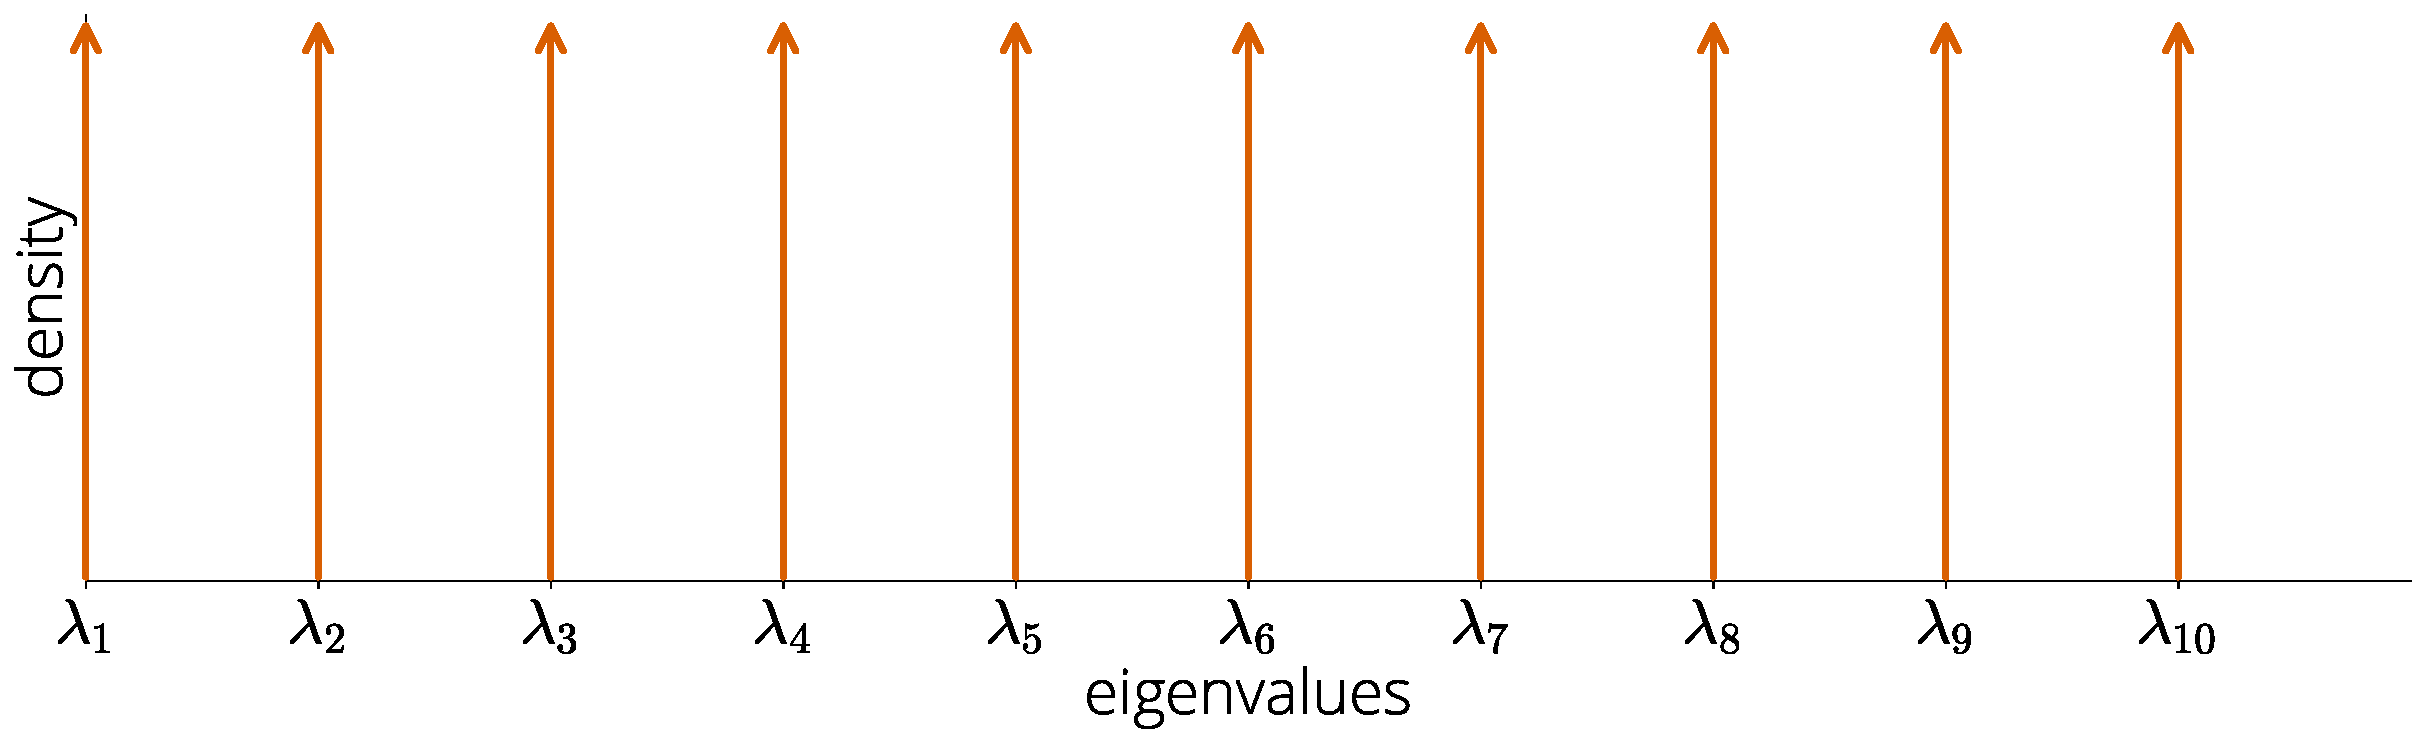
\includegraphics[width=0.8\linewidth]{part-1-images/esd.pdf}
\end{center}
\end{frame}
\begin{frame}{Wigner Semicircle Law}
\metroset{block=fill}
$\mu_{\text{ESD}}$  converges as $n \to \infty$ to the semicircular distribution, 
  \[ \mu_{\text{SC}}(x) \defas {\color{myorange}\frac{1}{2\pi} \sqrt{(4-x^2)_+} \, \dif x}\,.  \]

\centering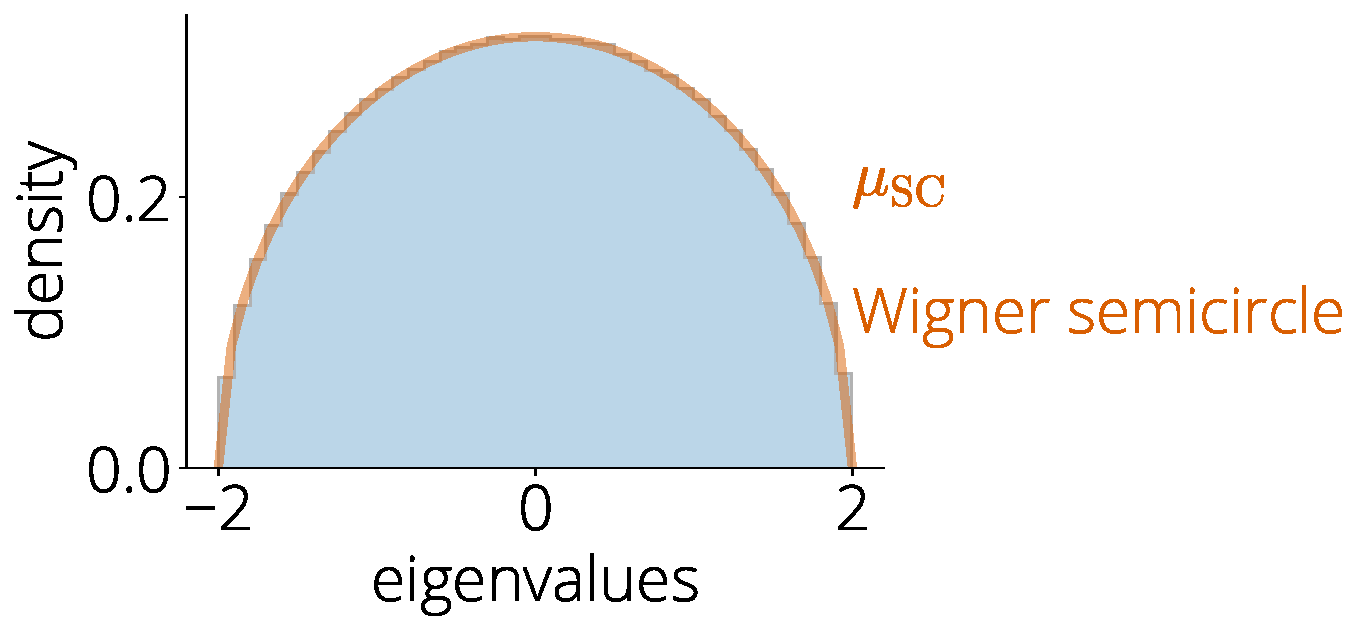
\includegraphics[width=0.6\linewidth]{part-1-images/wigner_semicircle.pdf}

{\footnotesize To know more: \citep{tao2012topics, bai2010spectral}.}
% \begin{center}
% \fcolorbox{blue}{white}{\parbox{0.8\textwidth}{
% \textcolor{red}{Converges:} If $\varphi : \mathbb{R} \to \mathbb{R}$ is bounded and continuous, 
% \[ \frac{1}{n} \sum_{i=1}^n \varphi\left (\lambda_i \left ( {\AA_n}\right ) \right ) \, \Prto{n} \,   \int_{\RR} \varphi(x) \mu_{\text{SC}}(\dif x) \]
% }}
% \end{center}
% \pause
% \vspace{0.1cm}

% \textcolor{red}{Do we need this ?}

% \begin{alertblock}{Moments of GOE, $\textcolor{red}{\GG_n}$}
% \begin{itemize}
%     \item {\small \textbf{1st moment:} $\text{tr}( \textcolor{red}{\GG_n} / 2\sqrt{n}) = \frac{1}{n} \sum_{i=1}^n \lambda_i ( \textcolor{red}{\GG_n} / 2\sqrt{n}) \Prto{n} \frac{2}{\pi} \int_{-1}^1 \textcolor{red}{x} \sqrt{1-x^2} \dif x = 0 $}\\~\\
%     \item { \small \textbf{2nd moment:} $\text{tr}( ( \textcolor{red}{\GG_n} / 2\sqrt{n})^2) = \frac{1}{n} \sum_{i=1}^n \lambda_i^2 ( \textcolor{red}{\GG_n} / 2\sqrt{n}) \Prto{n} \frac{2}{\pi} \int_{-1}^1 \textcolor{red}{x^2} \sqrt{1-x^2} \dif x = \frac{1}{4} $}
% \end{itemize}
% \textbf{Moment Method:} Knowing the moments \quad $\Rightarrow$ \quad density
%\end{alertblock}

\end{frame}

% \begin{frame}{Universality preview}
%     \note{In the previous computation we filled the matrix with elements from a Normal distribution, but, what happens if we choose a different distribution? Say, for example, a Bernouilli distribution (which was the one originally chosen by Wigner}
%     TODO: repeat experiment with Bernouilly RV
    
% \end{frame}

\begin{frame}[fragile]{Wishart ensemble}
    \metroset{block=fill}
 \begin{alertblock}{Wishart} 
\begin{itemize}
    \item $\XX$ = random $(d \times n)$ matrix with entries i.i.d. $\mathcal{N}(0,1)$
    \item Wishart ($d \times d$) matrix, $\WW = \frac{\XX \XX^T}{n}$
\end{itemize}
\end{alertblock}

\vspace{0.25cm}
\metroset{block = transparent}
 \begin{exampleblock}{Remarks}
 \begin{itemize}
     \item $\WW$ is symmetric, positive semi-definite
     \pause\item Same non-zero eigenvalues than $\frac{1}{n}\XX^T \XX$
     \pause\item$\frac{1}{n}\XX^T \XX$ is Hessian of the least squares problem $\frac{1}{2 n}\|\XX w - \yy\|^2$
     \pause\item Parameter ${\color{mybrown}\boldsymbol r} = \frac{d}{n}$
\end{itemize}
 \end{exampleblock}
 
 
\end{frame}

\begin{frame}[fragile]{Wishart ensemble}
  \begin{columns}
  \begin{column}{0.5\linewidth}
  \begin{exampleblock}{Python pseudocode}
    \begin{minted}[fontsize=\footnotesize]{python}
    import numpy as np
    import matplotlib.pyplot as plt

    r = 1/2  # for example
    X = np.random.randn(n * r, n)
    W = np.dot(X, X.T) / n
    
    eig = np.linalg.eigvals(W)
    plt.hist(eig)
    \end{minted}
    \end{exampleblock}
  \end{column}
  \begin{column}{0.5\linewidth}
    \includegraphics<1>[width=\linewidth]{part-1-images/wishart_1.pdf}
    \includegraphics<2>[width=\linewidth]{part-1-images/wishart_2.pdf}
    \includegraphics<3>[width=\linewidth]{part-1-images/wishart_3.pdf}
    \includegraphics<4>[width=\linewidth]{part-1-images/wishart_4.pdf}
    \includegraphics<5>[width=\linewidth]{part-1-images/wishart_5.pdf}
    \includegraphics<6>[width=\linewidth]{part-1-images/wishart_6.pdf}
  \end{column}
\end{columns}
\end{frame}

\begin{frame}{Limit of Wishart matrices}
    \begin{exampleblock}{Marchenko-Pastur (MP) law \citep{marvcenko1967distribution} }
     As $n, d \to \infty, \frac{d}{n} \to {\color{mybrown}\boldsymbol r}$, $\mu_{\text{ESD}}$ converges to the Marchenko-Pastur distribution:
    \begin{align*}
             {\color{myorange}{\boldsymbol\mu}_{\text{MP}}(x) \defas \underbrace{(1 - \tfrac{1}{{ r}})_+\delta_0(x)}_{\text{nonzero if ${\color{mybrown}\boldsymbol r} > 1$}} + \frac{\sqrt{({{\lambda}^+} - x)(x - {{\lambda}^-})}}{2 \pi {\color{mybrown}\boldsymbol r}\, x}1_{x \in [\lambda^-, \lambda^+]}\dif x\,.}\\
             \text{ with }  \lambda^- = (1 - \sqrt{\color{mybrown}\boldsymbol r})^2, {\lambda^+} = (1 + \sqrt{{\color{mybrown}\boldsymbol r}})^2
    \end{align*}
    \end{exampleblock}
    
    \begin{center}
    \vspace*{-0.5em}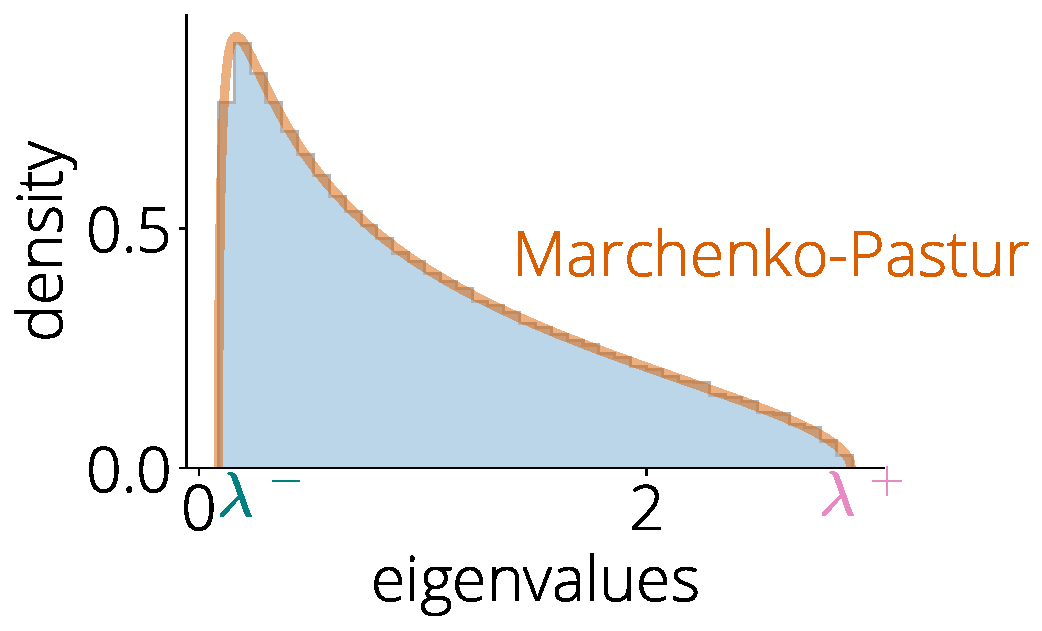
\includegraphics[width=0.4\linewidth]{part-1-images/MP.pdf}
    \end{center}
\end{frame}

\begin{frame}{The $r = \frac{d}{n}$ parameter}
\begin{itemize}
    \item $\textcolor{mybrown}{\boldsymbol r} < 1 \implies d < n \implies \WW$ is product of two {\bfseries fat} matrices.
    \item $\textcolor{mybrown}{\boldsymbol r} > 1 \implies d > n \implies \WW$ is product of two {\bfseries thin} matrices  (rank-deficient).
\end{itemize}

\begin{columns}
\begin{column}{0.5\linewidth}
\vspace*{1em}\begin{center}
    \includegraphics<1>[width=\linewidth]{part-1-images/MP_r_0.pdf}
    \includegraphics<2>[width=\linewidth]{part-1-images/MP_r_1.pdf}
    \includegraphics<3>[width=\linewidth]{part-1-images/MP_r_2.pdf}
    \includegraphics<4>[width=\linewidth]{part-1-images/MP_r_3.pdf}
    \includegraphics<5>[width=\linewidth]{part-1-images/MP_r_4.pdf}
    \includegraphics<6>[width=\linewidth]{part-1-images/MP_r_5.pdf}
\end{center}
\end{column}
\begin{column}{0.4\linewidth}
    \begin{align*}
             {\color{myorange}{\boldsymbol\mu}_{\text{MP}}(x) \defas \underbrace{(1 - \tfrac{1}{{ r}})_+\delta_0(x)}_{\text{nonzero if ${\color{mybrown}\boldsymbol r} > 1$}} + \frac{\sqrt{({{\lambda}^+} - x)(x - {{\lambda}^-})}}{2 \pi {\color{mybrown}\boldsymbol r}\, x}1_{x \in [\lambda^-, \lambda^+]}\dif x\,.}
    \end{align*}
\end{column}
\end{columns}
\end{frame}




% \section{Universality}

\begin{frame}{Universality}
\begin{exampleblock}{Covariance matrices $\WW = \frac{1}{n}\XX \XX^\top$}
What happens if we replace the $\mathcal{N}(0, 1)$ with a different distribution?
\begin{itemize}
    \item $X_{ij} \sim \mathcal{N}(0, 1)$
    \item \textcolor{myorange}{$X_{ij} \sim$ Rademacher $\Pr(X_{ij} = -1) = \Pr(X_{ij} = 1) = \frac{1}{2}$}
\end{itemize}
\end{exampleblock}
\pause
\begin{center}
    \includegraphics<2>[width=0.4\linewidth]{part-1-images/universality_0.pdf}
    \includegraphics<3>[width=0.4\linewidth]{part-1-images/universality_1.pdf}
    \includegraphics<4>[width=0.4\linewidth]{part-1-images/universality_2.pdf}
    \includegraphics<5>[width=0.4\linewidth]{part-1-images/universality_3.pdf}
    \includegraphics<6>[width=0.4\linewidth]{part-1-images/universality_4.pdf}
\end{center}
\end{frame}


% in most cases, it is possible to replace the original distribution with a (appropriately normalized) Gaussian distribution
\begin{frame}{Universality}
\begin{exampleblock}{Universality}
\begin{itemize}
\item Statistics only mildly  depend on the lower order moments of distribution of the entries 
    % \item Eigenvalue distributions \, $\Rightarrow$ \,  \textcolor{red}{central limit theorem}
\end{itemize}
\end{exampleblock}
\pause
\vspace{0.1cm}

\metroset{block = fill}
\begin{exampleblock}{Example: Marchenko-Pastur \citep{marvcenko1967distribution}} Let $\XX$ be a $d \times n$ random matrix with i.i.d. entries that verifies
\begin{table}[]
    \centering
    \begin{tabular}{c c c}
        $\mathbb{E}[X_{ij}] = 0$,\quad $\mathbb{E}[X_{ij}^2] = 1$,\quad $\mathbb{E}[X_{ij}^4] < \infty$   
    \end{tabular}
\end{table}
{\bfseries Universality:} \quad As $n, d \to \infty$ with $\frac{d}{n} \to {\color{mybrown}\boldsymbol r}$, the ESD of $\WW = \frac{\XX \XX^T}{n}$ converges to Marchenko-Pastur(${\color{mybrown}\boldsymbol r}$)
\end{exampleblock}

% \pause
% \begin{center}
% Things become simple in high dimensions
% \end{center}
\end{frame}


\begin{frame}{May others ...}
\begin{exampleblock}{Other matrix ensembles}
\begin{itemize}
    \item {\bfseries Ginibre.} Let $\GG_n$ be $n \times n$ matrix of i.i.d. $N(0,1)$, {\footnotesize(bilinear games \citep{domingo2020average})}
    \[\text{(Circle law)} \quad \text{ESD of $\GG_n/\sqrt{n} \to \text{Unif}(\text{disk})\,.$}\]
    \item 
    Uniform probability measure on {\bfseries orthogonal matrices}. $\VV \sim \text{Unif}(O(n))$,
    \[  \text{ESD of $\VV$} \to  \text{Unif}(\mathbb{S}^1)\,.\]
\end{itemize}
\end{exampleblock}

\begin{center}
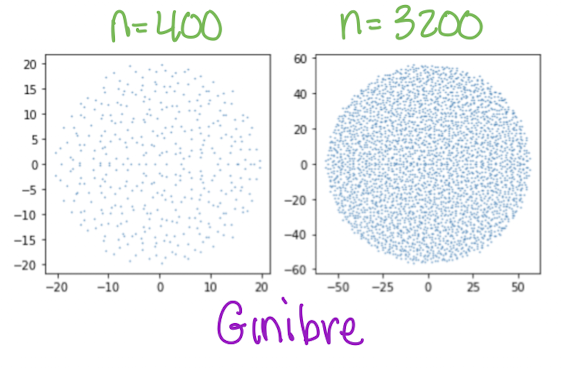
\includegraphics[scale = 0.5]{part-2-images/Ginibre.png}\hspace{0.2cm} 
    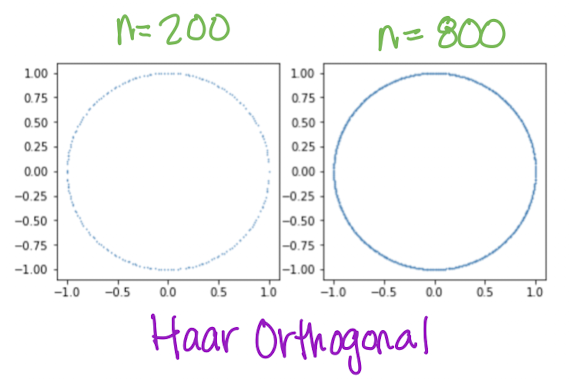
\includegraphics[scale = 0.5]{part-2-images/Haar.png} 
\end{center}
\end{frame}


\appendix



\begin{frame}[allowframebreaks]{References}

  \bibliographystyle{plainnat}
  {\scriptsize\bibliography{references}}

\end{frame}

\end{document}
